\cleardoublepage
\chapter{Diseño e implementación}
\label{chap:design_implement}



En este capítulo se realiza una descripción detallada sobre el diseño y la implementación del presente Trabajo de Fin de Grado.


La arquitectura de la aplicación esta diferenciada en el lado del cliente y en el lado del servidor aunque interactúan entre ellos. El cliente está desarrollado con las tecnologías HTML5, CSS3, JavaScript, BootStrap, jQuery, mientras que el servidor se desarrolla en Python, Django y Mezzanine.



\section{Arquitectura general} 
\label{sec:arquitectura}

FIXME: estaría bien tener un esquema de la arquitectura general en un diagrama.

El proyecto consta de múltiples ficheros y directorios. Aunque se haya utilizado un CMS, la arquitectura sigue siendo la misma que la utilizada en Django. Cada una de las distintas aplicaciones que contiene el presente proyecto mantiene la siguiente estructura:
\begin{itemize}
\item Urls.py: es la interfaz entre el cliente y el servidor. Maneja las peticiones HTTP recibidas y las envía a la función contenida en el \textit{views} correspondiente.
\item Views.py: recibe la información de la petición HTTP y devuelve una respuesta. En el presente proyecto sólo se reciben peticiones GET y peticiones POST.
\item Models.py: determina la estructura de datos.
\item Templates: contiene las plantillas HTML que definen la interfaz de usuario
\item Static: contiene los ficheros estáticos CSS y JS, además de contener las imágenes utilizadas.
\item Utils: contiene funciones llamadas por el \textit{views}. Cada llamada recibe unos parámetros, los procesa y devuelve un resultado fruto de ese procesamiento.
\end{itemize}


Como se ha comentado anteriormente, cuando el servidor recibe una petición HTTP por parte del cliente, dicha petición es manejada desde el fichero principal urls.py. Tras encontrar la URL en dicho fichero continúa con el siguiente fichero urls.py (que será el de la aplicación pedida) a continuación se hace ejecutar la función correspondiente del fichero views.py. La función trata la petición GET o POST y responderá con una petición HTTP que devolverá la plantilla HTML (con todos los demás ficheros estáticos) correspondiente al cliente.


\section{Diseño e implementación del servidor} 
\label{sec:servidor}


\subsection{Modelos de la base de datos} 
\label{subsec:modelos}


La aplicación requiere una base de datos donde se guardará toda la información que los usuarios introduzcan en la aplicación web. La estructura de la base de datos se almacena, como hemos comentado antes, en el archivo models.py (como hemos dicho anteriormente, cada aplicación contiene su propio archivo models.py). Django generará las tablas pertinentes dentro de la base de datos. La base de datos utilizada es SQLite3 que es un tipo de base de datos relacional.


La ventaja que tenemos al usar un Django es que la conexión con los sistemas de la base de datos es transparente para el usuario. 

 \begin{figure}[H]
    \centering
    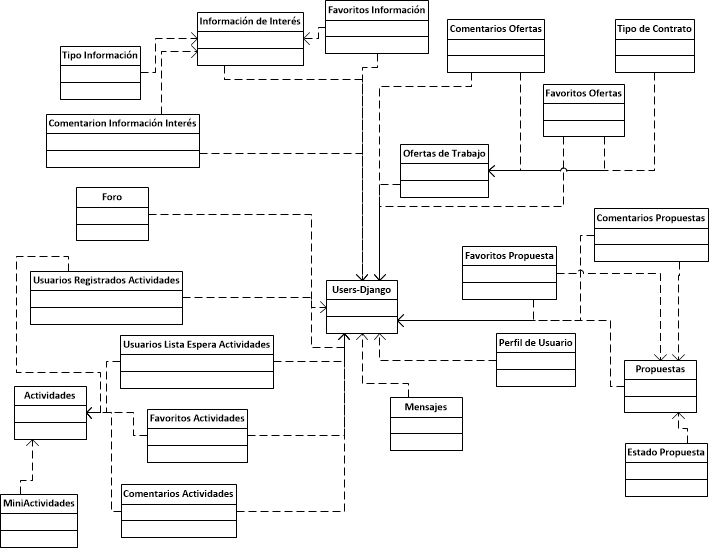
\includegraphics[width=12cm]{img/bbdd}
    \caption{Base de datos}
    \label{figura:base_datos}
 \end{figure}

FIXME: la figura queda un poco rara, porque no se pueden ver los campos de cada tabla.
 

A continuación se enumeran y describen cada una de las aplicaciones que utilizan la base de datos mostrada en la figura 1:


\begin{itemize}
\item Theme: en esta aplicación se define la estructura que tendrá la \textit{homepage}, también incluyen modelos para la creación de FAQs y la creación de un blog y sus respectivas entradas.
\item Propuestas: con esta aplicación conseguimos que los usuarios propongan sus propias actividades o al tipo de actividades que desean asistir.
\item Ofertas: con esta aplicación conseguimos dar a conocer las ofertas de trabajo y prácticas en empresas.
\item Actividades: con esta aplicación conseguimos dar a conocer las distintas actividades que se realizan en la Universidad. Estas actividades van desde un simple seminario o charla hasta actividades un poco más grandes como podría ser un taller con varios seminarios dentro o incluso la organización y difusión de la semana de San Teleco. 
\item Información de interés: con esta aplicación conseguimos difundir el resto de información que se desee compartir como becas, cursos, concursos, etc. 
\item Perfil: con esta aplicación conseguimos complementar el modelo de usuario creado por Django.
El modelo de Perfil creado debe referenciar a un usuario, pero no puede existir más de un perfil por usuario. 
No se mostrará públicamente algunos datos de carácter personal debido a la ley de protección de datos.
\item BasicModels y BasicContent: estas dos aplicaciones han sido creadas para proporcionar una base para dos propósitos:
\begin{itemize}
\item Crear páginas básicas como las creadas para mostrar las listas de ofertas, información de interés, etc.
\item o	Extender el modelo al crear los modelos anteriormente comentados unificando en uno solo los campos comunes, además de proporcionar \textit{templates} comunes para el resto de aplicaciones.
Con estas dos aplicaciones conseguimos reducir el código, evitando en la medida de lo posible la repetición del mismo.
\end{itemize}
\end{itemize}


\subsection{Tipo de usuarios} 
\label{subsec:usuarios}


Dentro de la aplicación se distinguen tipos de usuarios, con distintos roles y diferentes permisos:

\begin{itemize}
\item No registrados: Estos usuarios sólo pueden ver el contenido de la aplicación pero no pueden interactuar ni con la aplicación ni con otros usuarios.
\item Alumnos: Este tipo de usuarios además de ver el contenido, pueden interactuar con la aplicación, lo único que no pueden hacer es crear actividades, aunque podrían editarlas y eliminarlas si formaran parte de la administración en alguna de ellas.
\item Profesores: Este tipo de usuarios además de lo que los alumnos pueden hacer también pueden crear actividades y cambiar el estado de una propuesta.
\item Administradores: Además de todo lo descrito anteriormente. Tiene acceso a la parte de administración.
\end{itemize}


\subsection{Amazon Web Service + Apache} 
\label{subsec:aws_apache}

La aplicación se ha desplegado en una máquina EC2 de Amazon Web Service usando una cuenta gratuita para estudiantes de duración de un año.

Para crear la máquina se ha escogido las siguientes opciones:
\begin{itemize}
\item El sistema operativo es: Ubuntu 14.04 LTS con una capacidad total de 8GB.
\item Una instancia de tipo t2.micro: 1 GiB de memoria, 1 vCPU solo para EBS y plataforma de 32 bits o 64 bits. Las instancias T2 son instancias de desempeño con ráfagas que proporcionan un nivel base de desempeño de la CPU con la posibilidad de alcanzar ráfagas por encima del nivel básico. Las instancias de este tipo son ideales para aplicaciones que no usan la CPU por completo, a menudo o de manera constante, pero que de vez en cuando tienen que alcanzar ráfagas (por ejemplo, servidores web, entornos para desarrolladores y bases de datos). En este caso es una máquina de 64bits.
\end{itemize}

En las siguientes imágenes se pueden ver las diferentes características de la máquina creada:

\begin{figure}[H]
   \centering
   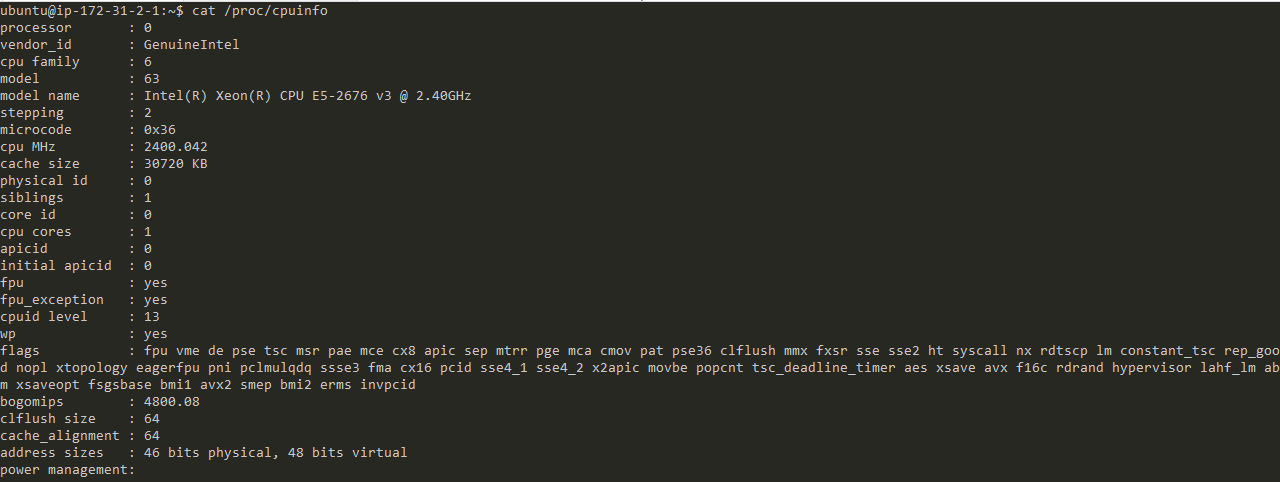
\includegraphics[width=12cm]{img/cpuinfo}
   \caption{Salida de la ejecución del comando cat /proc/cpu/info }
   \label{figura:cpuinfo}
\end{figure}
\begin{figure}[H]
   \centering
   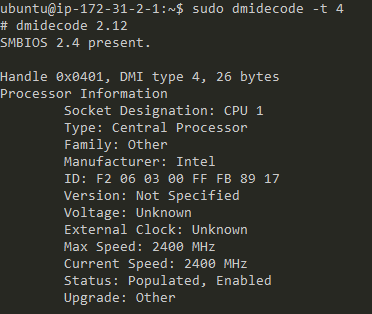
\includegraphics[width=12cm]{img/dmidecode}
   \caption{Salida de la ejecución del comando sudo demidecode -t 4}
   \label{figura:dmidecode}
\end{figure}
\begin{figure}[H]
   \centering
   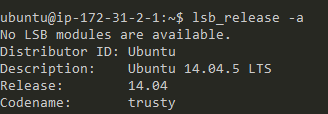
\includegraphics[width=12cm]{img/lsb_release}
   \caption{Salida de la ejecución del comando lsb\_release -a}
   \label{figura:lsb_release}
\end{figure}
\begin{figure}[H]
   \centering
   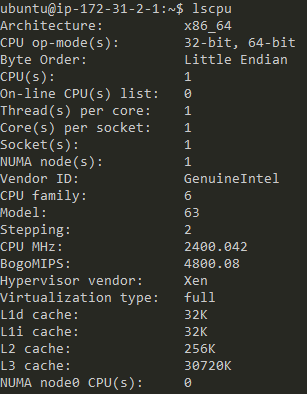
\includegraphics[width=12cm]{img/lscpu}
   \caption{Salida de la ejecución del comando lscpu}
   \label{figura:lscpu}
\end{figure}
\begin{figure}[H]
   \centering
   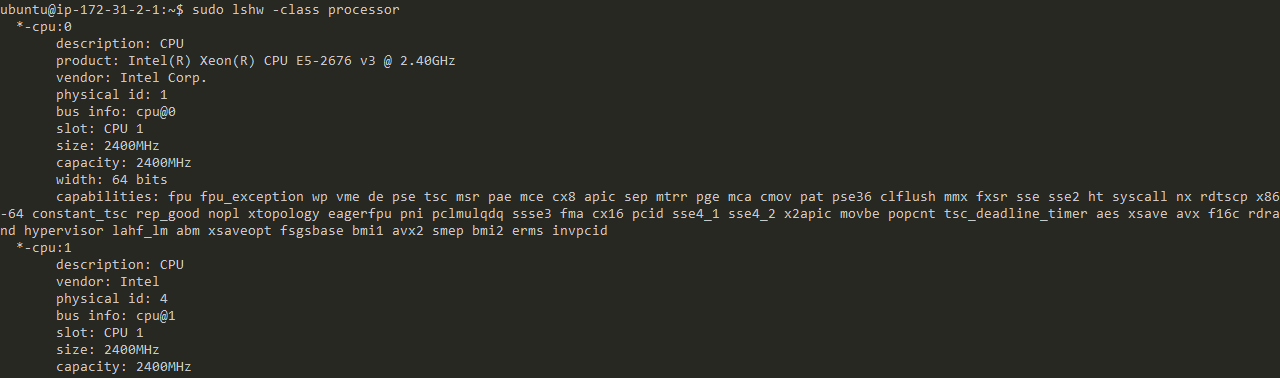
\includegraphics[width=12cm]{img/lshw}
   \caption{Salida de la ejecución del comando lshw}
   \label{figura:lshw}
\end{figure}
\begin{figure}[H]
   \centering
   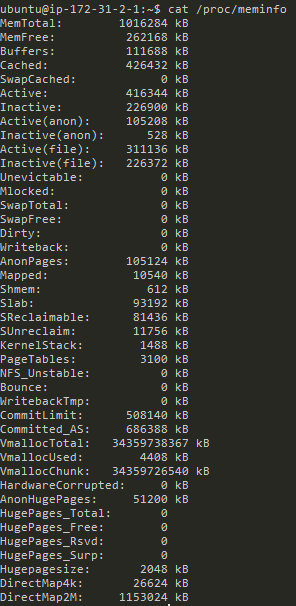
\includegraphics[width=12cm]{img/meminfo}
   \caption{Salida de la ejecución del comando cat /proc/meminfo}
   \label{figura:meminfo}
\end{figure}


Para la configuración de Apache, primero se debe instalar usando el comando: 

\begin{verbatim}
	apt-get install apache2
\end{verbatim}

Para poder servir aplicaciones Django desde un servidor Apache, lo más habitual es añadir el módulo mod\_wsgi, que permite servir aplicaciones hechas en Python, que tengan soporte para la interfaz WSGI (Como es el caso de Django y en este caso también de Mezzanine).


Para ello se instala el paquete del repositorio:
\begin{verbatim}
	sudo apt-get install libapache2-mod-wsgi
\end{verbatim}

A continuación se configuró el host virtual de Apache. Un virtual host permite mantener múltiples nombres de host en Apache. Gracias a ello, se puede decirle a Apache que redirija las peticiones procedentes de una URL determinada, a una aplicación concreta.

Para generar la configuración del host virtual, se creó un archivo en /etc/apache2/sites-available/ con el nombre de Welpe.

La configuración usada se muestra en la siguiente captura:

\begin{figure}[H]
   \centering
   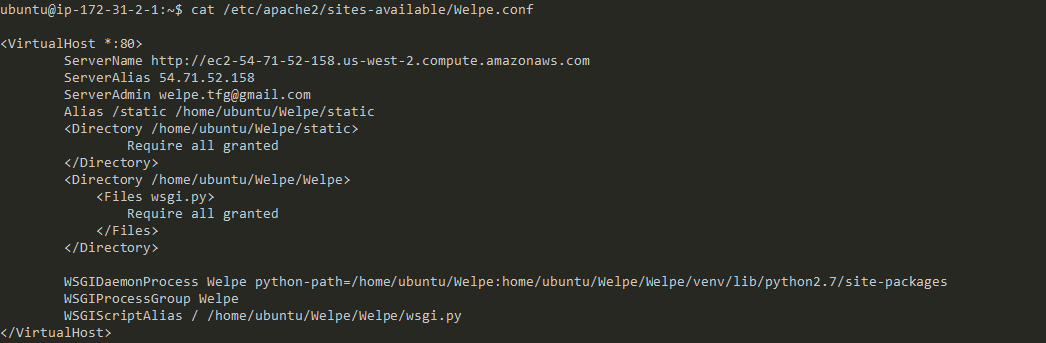
\includegraphics[width=12cm]{img/welpe_conf}
   \caption{Fichero de configuración en Apache}
   \label{figura:welpe_conf}
\end{figure}

Después de configurar el anterior fichero, se activó el host virtual y se reinició el servidor mediante:
\begin{verbatim}
	sudo a2ensite Welpe
	sudo /etc/init.d/apache2 restart
\end{verbatim}


\section{Diseño e implementación del cliente} 
\label{sec:cliente}


El cliente puede acceder a la interfaz web a través de un navegador web. Como bien se ha comentado anteriormente, se han utilizado distintas tecnologías para que la interfaz sea más amigable. HTML5 y CSS3 junto con Bootstrap y jQuery han sido necesarias para definir cómo se visualizan y con qué estilos y diseños aparecen cada uno de los elementos visibles en esta aplicación. 

Estaría bien un diagrama con las vistas que tiene.


Todas las vistas de este proyecto siguen el mismo esquema:

FIXME: estaría bien tener este esquema en un diagrama.


\begin{itemize}
\item Una barra superior o \textit{header} que consta del logotipo de la aplicación junto con el login y un formulario de búsqueda. Además también consta del menú y ya por último se ha introducido también otra pequeña cabecera con el nombre de vista junto con lo que llamaríamos \textit{breadcrumb} o migas de pan.  Breadcrumb es un elemento que aporta al usuario la información de dónde se encuentra en cada momento dentro de un sitio web. Se indica la ubicación exacta de la página y la relación jerárquica de esta con respecto a la de inicio del sitio web.
\item Contenido principal de la página. En esta sección lo que nos encontramos es con el contenido renderizado que estamos pidiendo a través de la URL introducida ya sea el perfil de usuario, una actividad, una oferta o cualquier otra petición.
\item Footer. En el footer podemos encontrar el copyright®, política de cookies, etc.
\end{itemize}


\subsection{Vistas de las páginas} 
\label{subsec:vistas}

A continuación se describen una a una todas las páginas de la aplicación explicando cada elemento que aparece en las páginas así como su utilidad. Todas las páginas en principio son públicas y accesibles para todo tipo de usuarios tanto para los registrados como para los no registrados aunque también se ha de decir, que estando registrado en esta aplicación, se puede interactuar por ejemplo escribiendo comentarios, creando propuestas, etc., además si en un futuro esta aplicación se expandiera podría tener contenido exclusivo sólo para usuarios registrados.


\subsubsection{Página de inicio}
\label{subsubsec:home}


La página de inicio es enviada al cliente cuando se recibe una petición GET sobre el recurso /, a través de la vista home. En esta vista hace un resumen de las características que tiene la aplicación web.

 \begin{figure}[H]
    \centering
    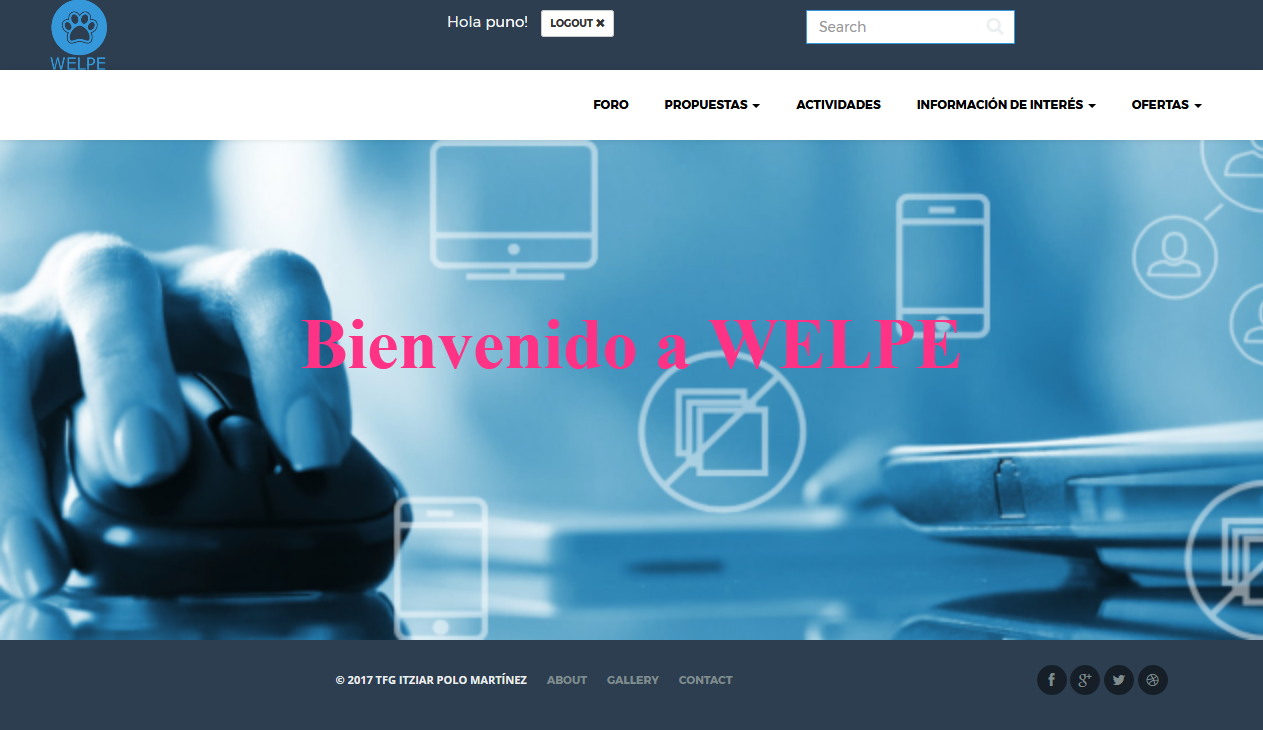
\includegraphics[width=12cm]{img/home}
    \caption{Hompage}
    \label{figura:home}
 \end{figure}
 
 
\subsubsection{Página del Perfil de Usuario}
\label{subsubsec:profile}

La página del perfil es enviada al cliente cuando se recibe una petición GET sobre el recurso /perfil/{id\_usuario}.


En esta vista se muestra la información de un usuario.


El contenido dependerá de si un usuario accede a su propio perfil o al perfil de otro usuario.


Aquí nos encontramos varias cosas:

\begin{itemize}
\item El perfil de usuario que además de la información del usuario, se podrá interactuar con él, enviándole un mensaje privado.
\item Si se accede al propio perfil, se podrá además de editarlo, tener acceso a la lista de mensajes tanto enviados como recibidos, a la lista de favoritos ordenados por cada uno de los eventos y ver las actividades en las que se desea participar.
\end{itemize}

 \begin{figure}[H]
    \centering
    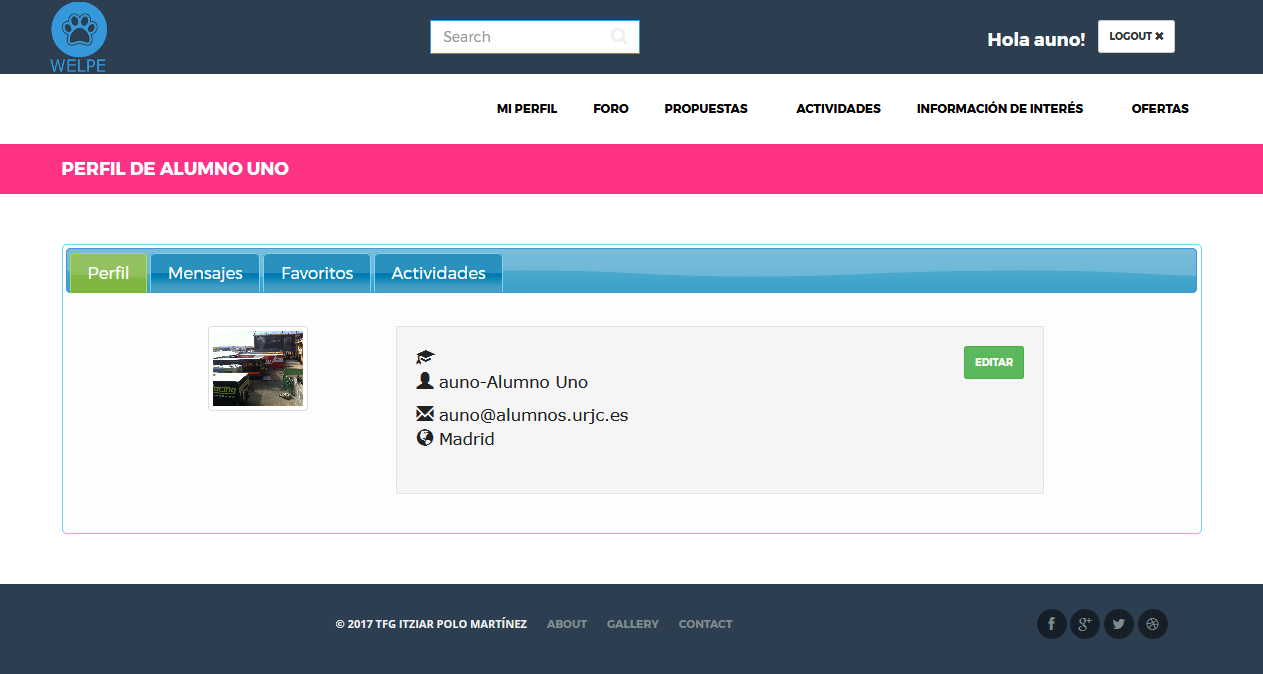
\includegraphics[width=12cm]{img/mi_perfil}
    \caption{Vista del perfil de usuario}
    \label{figura:perfil_usuario}
\end{figure}
\begin{figure}[H]
 \centering
 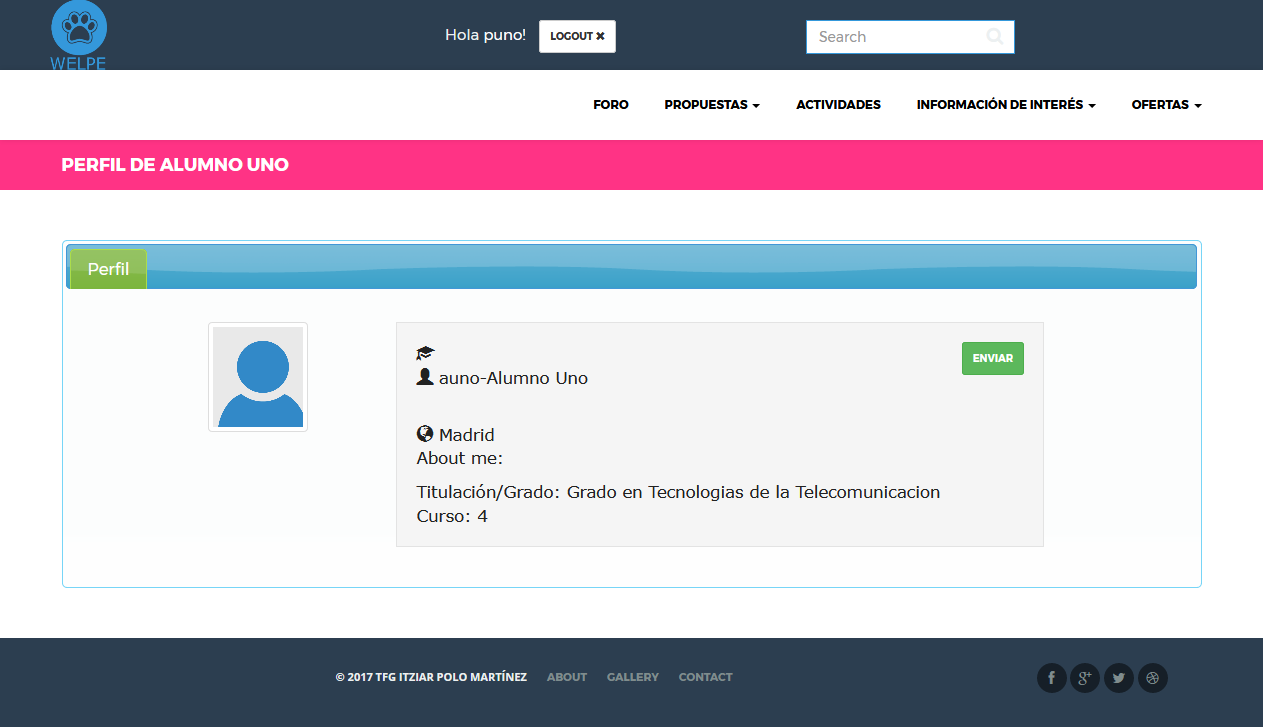
\includegraphics[width=12cm]{img/perfil_otro}
 \caption{Vista del perfil de otro usuario distinto}
 \label{figura:perfil_otro_usuario}
\end{figure}
\begin{figure}[H]
  \centering
  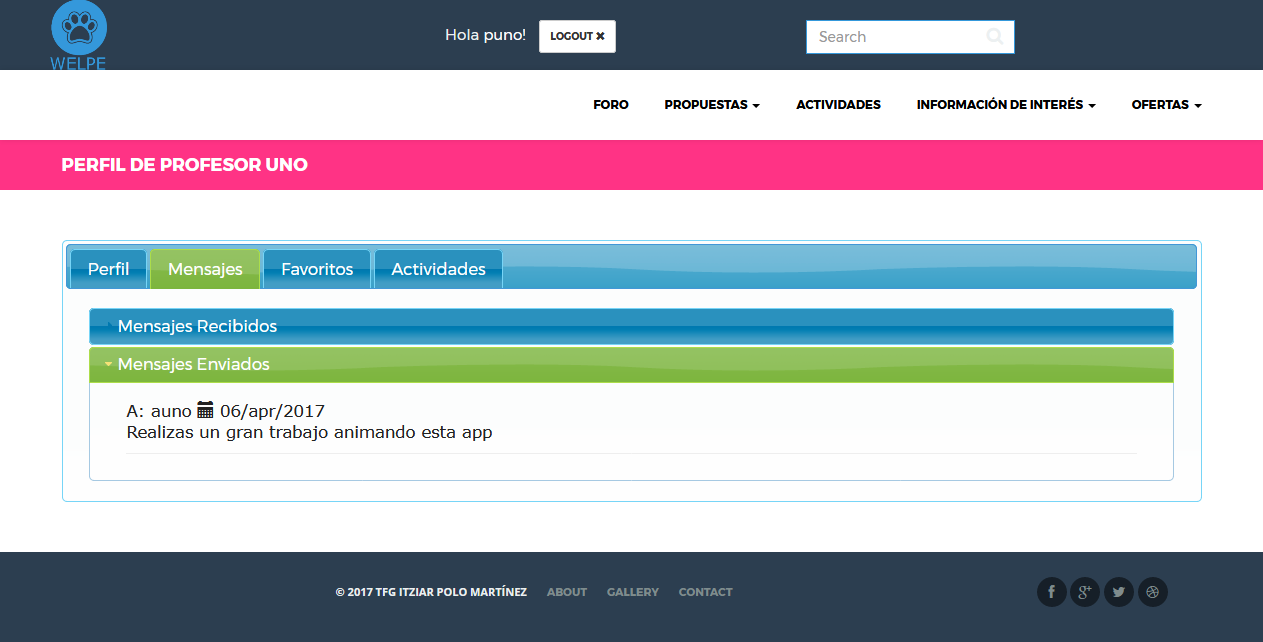
\includegraphics[width=12cm]{img/perfil_mensajes}
  \caption{Vista de los mensajes}
  \label{figura:perfil_mensajes}
\end{figure}
\begin{figure}[H]
   \centering
   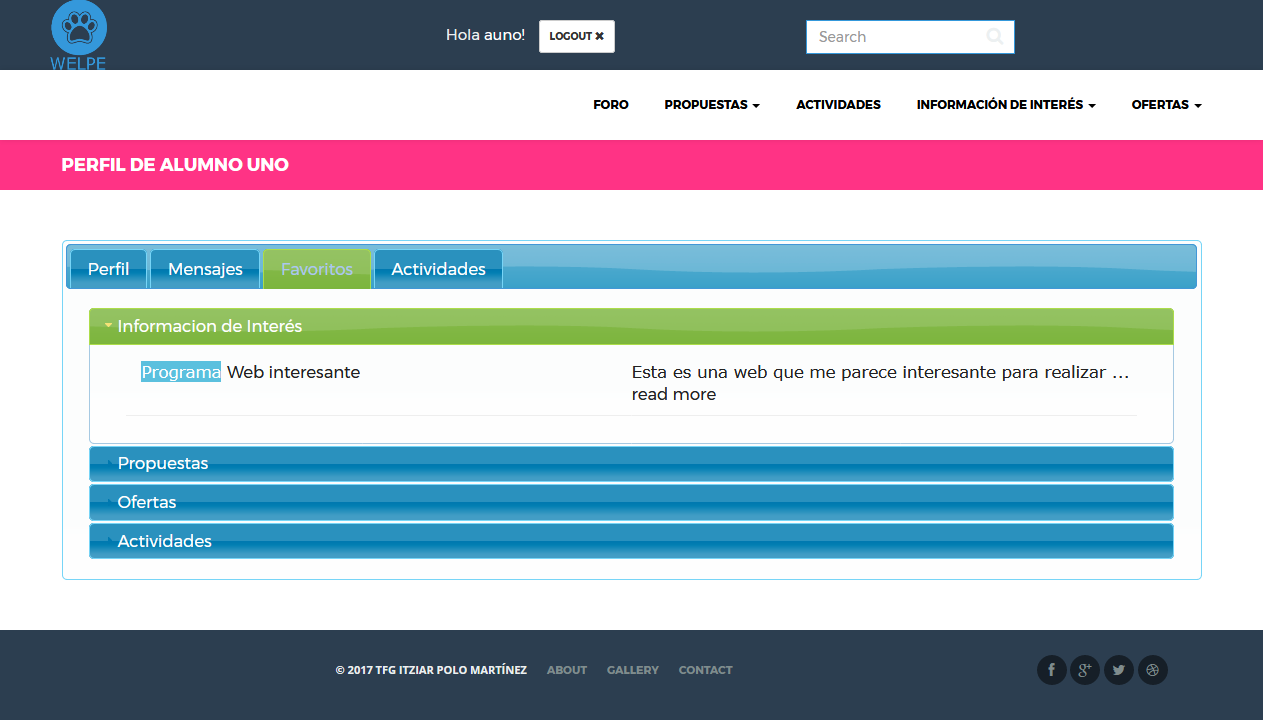
\includegraphics[width=12cm]{img/perfil_favoritos}
   \caption{Vista de favoritos}
   \label{figura:perfil_favoritos}
\end{figure}
\begin{figure}[H]
   \centering
   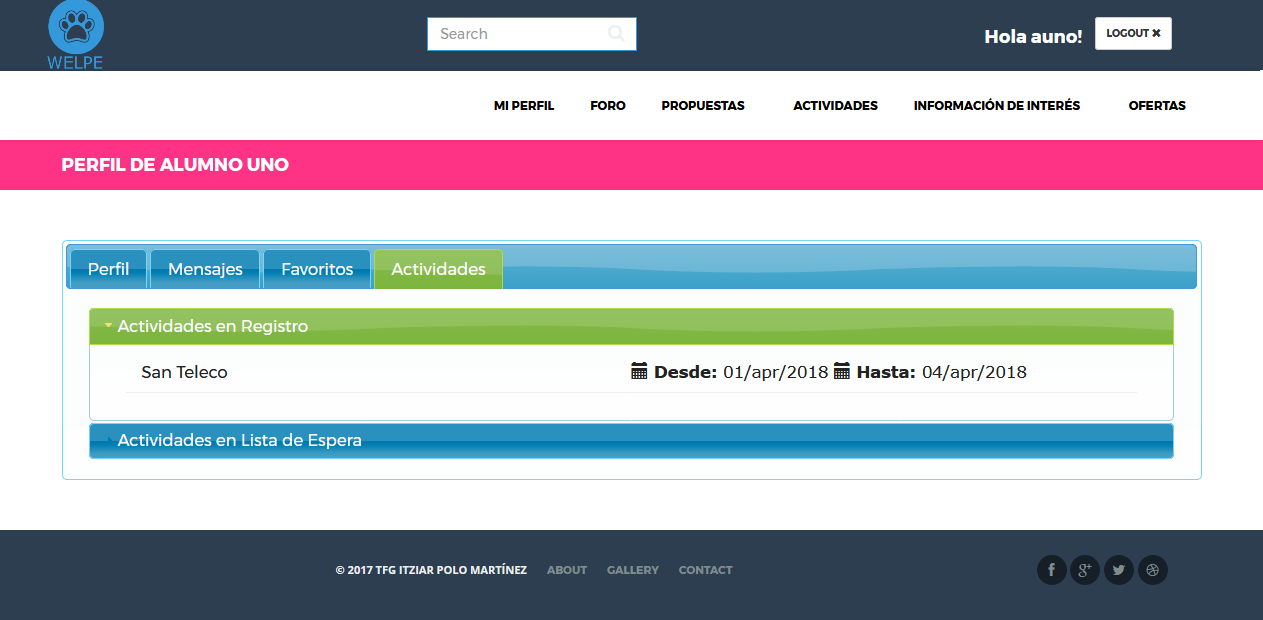
\includegraphics[width=12cm]{img/perfil_actividades}
   \caption{Vista de actividades registradas}
   \label{figura:perfil_actividades}
\end{figure}
        
        
\subsubsection{Página del Foro}
\label{subsubsec:foro}

La página del foro es enviada al cliente cuando se recibe una petición GET sobre el recurso /foro.


La página foro contiene todos los mensajes publicados en el foro.


Cada mensaje contiene la foto y el nombre del usuario (aunque estos datos pueden ser anónimos), la fecha en la que se publicó, un título de comentario, una descripción (que será opcional).


Encima de estos mensajes al igual que en las demás vistas que contienen comentarios aparece un formulario para si se desea dejar un comentario.

El objetivo inicial del foro era dotar a la aplicación de un aspecto más social según lo comentado en los objetivos.


La función del foro es la de conectar a todos los usuarios, permitiendo un entorno universitario conectado y permitiendo mejorar el mismo, por ejemplo compartiendo curiosidades que los usuarios vayan encontrando durante su estancia en la universidad.

\begin{figure}[H]
   \centering
   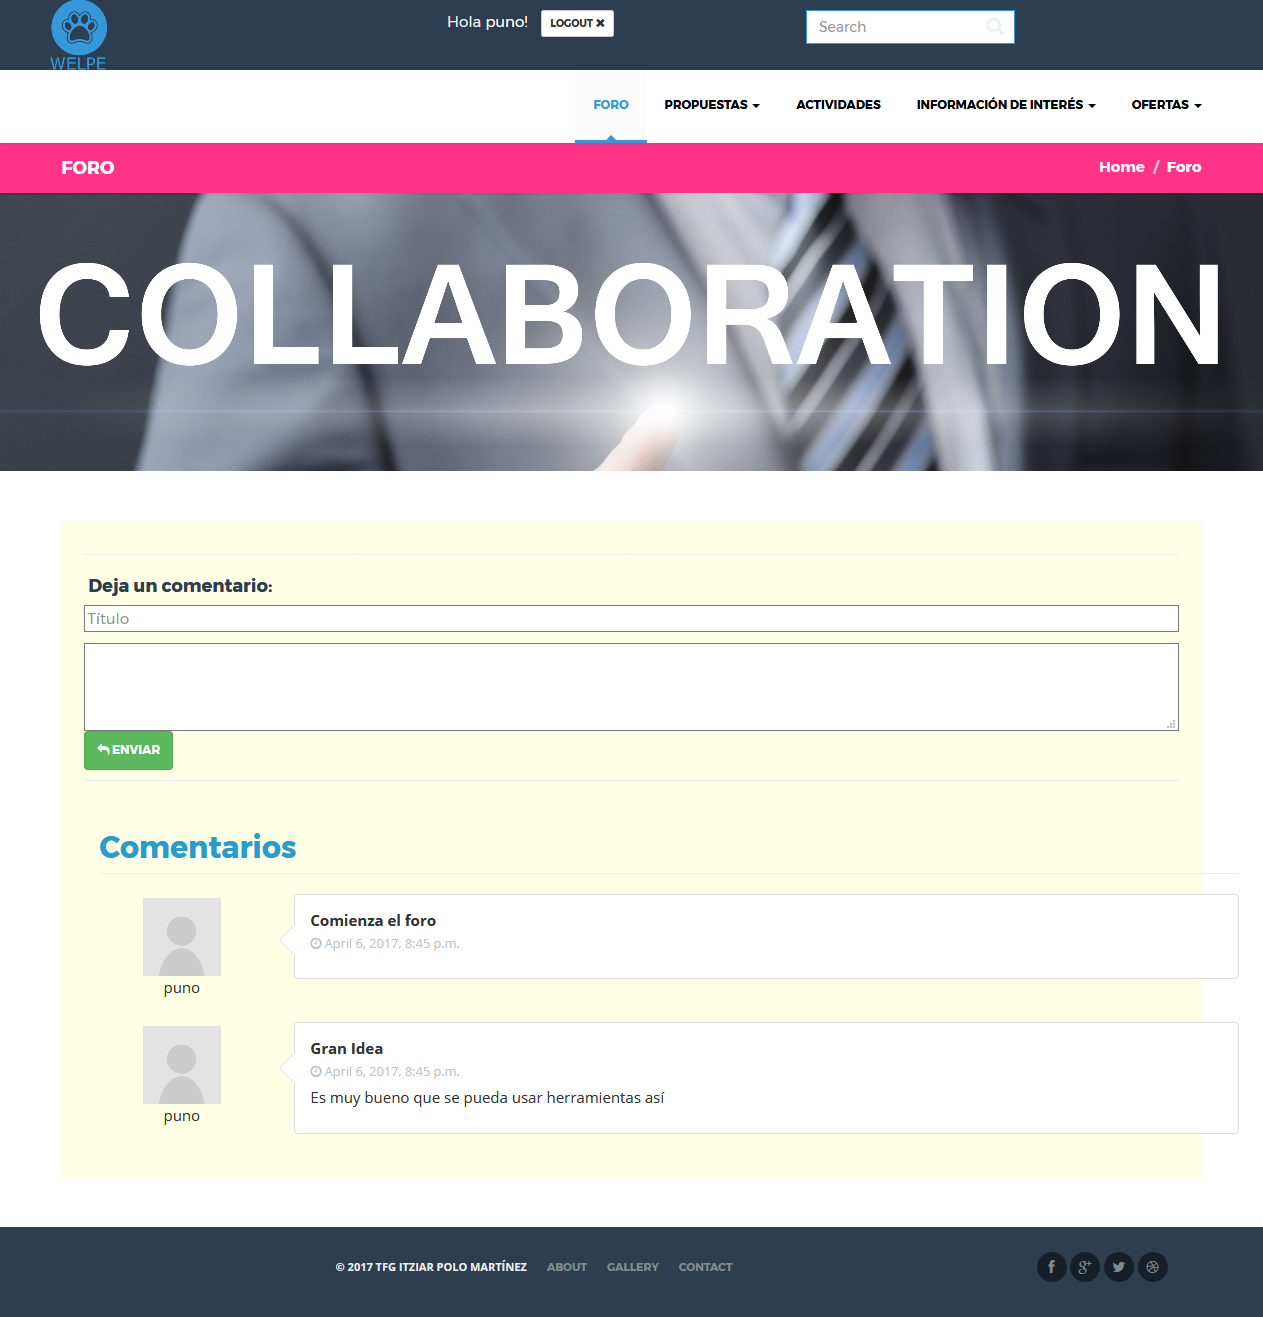
\includegraphics[width=12cm]{img/foro}
   \caption{Vista del foro}
   \label{figura:foro}
\end{figure}


\subsubsection{Página de Propuestas}
\label{subsubsec:propuestas}


La página del listado de propuestas es enviada al cliente cuando se recibe una petición GET sobre el recurso /propuestas.


En esta vista se proporciona un listado con todas las propuestas que se han ido recopilando, junto con una pequeña parte de la descripción. Además a la izquierda del título se muestra el estado de la propuesta y a la derecha se puede observar varios elementos. En primer lugar un corazón que viene a significar si la propuesta se ha guardado en la lista de favoritos o no, además de un número que irá creciendo o decreciendo dependiendo del número de usuarios la guarden en sus listas de favoritos. A continuación se observa el número de comentarios que contiene cada una de las ofertas.


También cualquier usuario (registrado o no) puede filtrar las propuesta por las palabras que contenga el título o contenido de la propuesta, además también se puede filtrar por el estado de las propuestas a elegir entre enviado, aceptado o rechazado, además si el usuario está registrado podrá filtrar si la propuesta está o no en su lista de favoritos.


Para introducir una nueva propuesta cualquier usuario registrado puede hacerlo. Para ello, se rellena el formulario con los datos correspondientes y envía ese formulario. Esta petición llega al servidor mediante una petición POST donde se encargará de sacar los datos y guardarlos correctamente en la base de datos, devolviendo como resultado una nueva vista donde se muestra la nueva propuesta.


Por último, sólo si el usuario ha creado una determinada propuesta o es un profesor o es el administrador: podrá modificar y/o eliminar dicha propuesta mediante los botones edit y delete.

\begin{figure}[H]
   \centering
   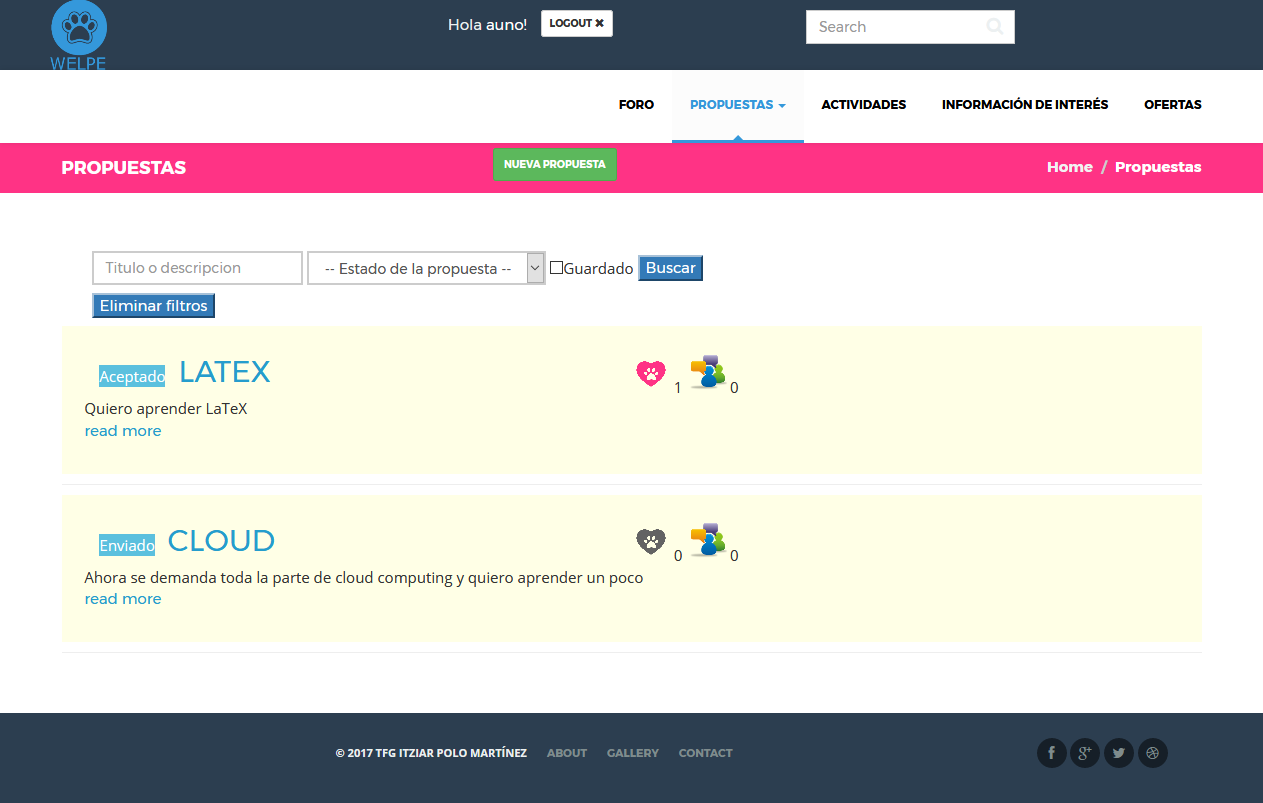
\includegraphics[width=12cm]{img/propuestas}
   \caption{Vista de la lista de propuestas}
   \label{figura:propuestas}
\end{figure}

\subsubsection{Página de una Propuesta}
\label{subsubsec:propuesta}


La página de una propuesta es enviada al cliente cuando se recibe una petición GET sobre el recurso /propuestas/{título\_propuesta}


En esta vista se muestra toda la información relativa a la propuesta previamente introducida a través del formulario comentado anteriormente. 


Relativo a esta vista, se encuentra el nombre, el estado de la propuesta, número de comentarios, los comentarios, la popularidad que se mide en el número de favoritos, etc.


En esta vista se puede interactuar de las siguientes formas sólo si es un usuario registrado:


\begin{itemize}
\item Se puede crear una nueva propuesta mediante el botón nueva propuesta donde se abrirá un modal en el que se pedirán ciertos datos; este formulario ya cumplimentado se enviará al servidor donde se procesará y almacenara devolviendo como resultado una nueva vista donde se muestra la nueva propuesta que el usuario ha creado.
\item Si el usuario es el propietario de la propuesta podrá modificarla mediante el botón edit y también podrá eliminarla mediante el botón eliminar.
\item Junto con todo ello, está también el botón de favoritos donde el usuario puede agregar o eliminar la propuesta de su lista de favoritos.  
\item Se ha proporcionado un apartado de comentarios a la propuesta para que los usuarios puedan comentar cada propuesta.
\item Sólo los profesores y el administrador pueden cambiar el estado de la propuesta. Esto es así, ya que el objetivo de las propuestas es que los alumnos den opinión de qué es lo que quieren aprender en los seminarios y/o proponer ellos mismos los seminarios que quieren impartir.
\end{itemize}

\begin{figure}[H]
   \centering
   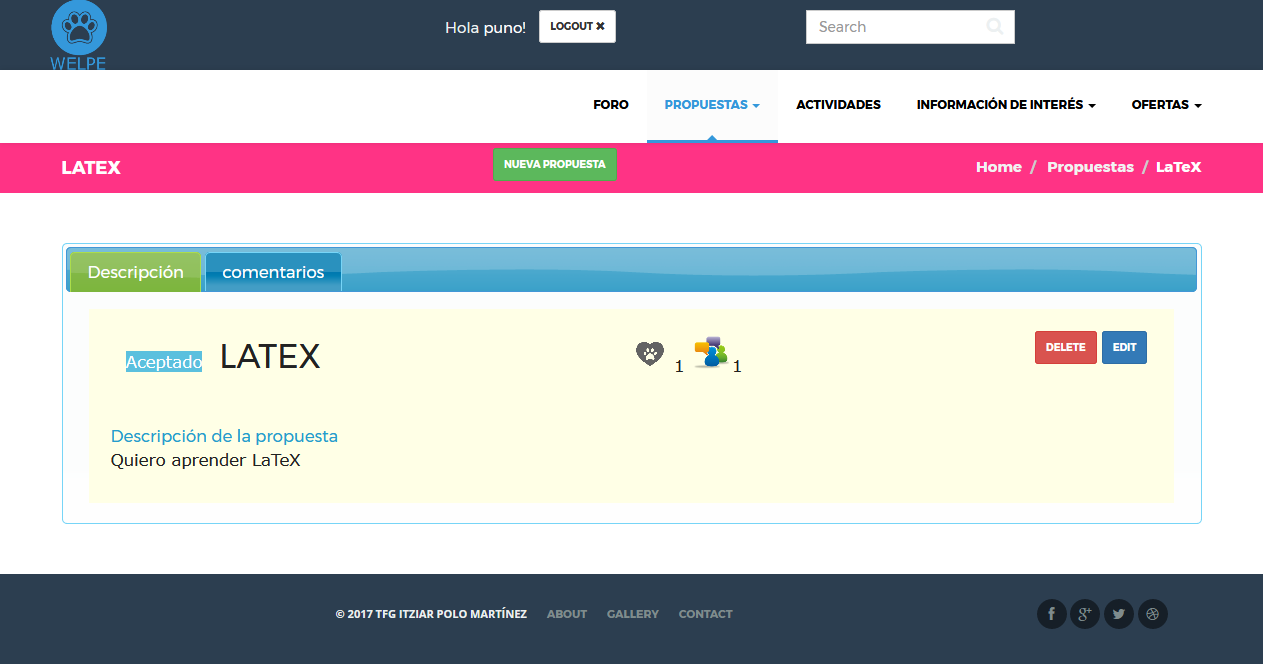
\includegraphics[width=12cm]{img/propuesta}
   \caption{Vista de una propuesta}
   \label{figura:propuesta}
\end{figure}

\begin{figure}[H]
   \centering
   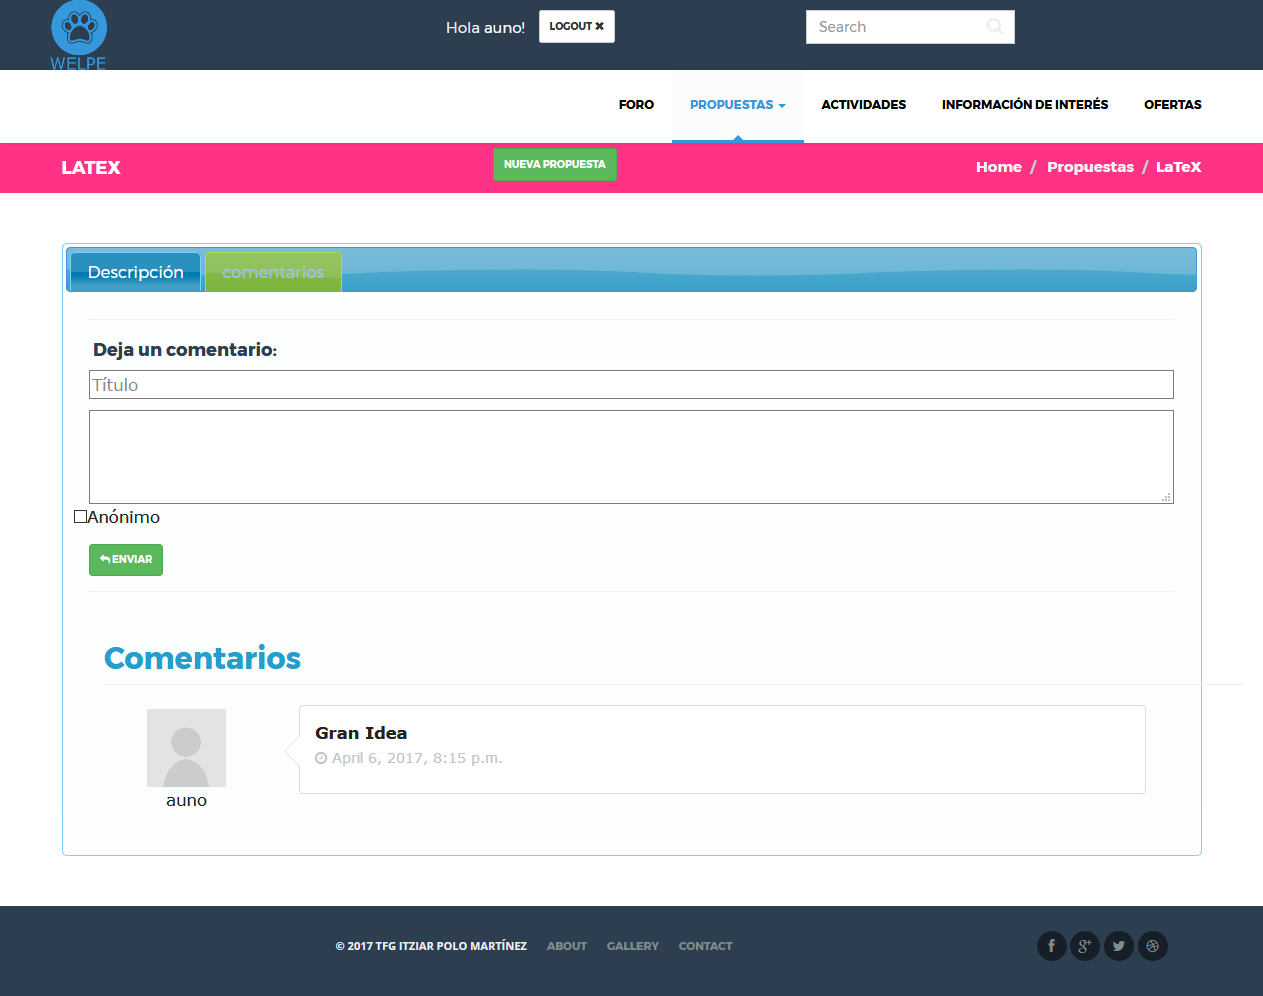
\includegraphics[width=12cm]{img/propuesta_comment}
   \caption{Vista de los comentarios a una propuesta}
   \label{figura:propuesta_comment}
\end{figure}

\subsubsection{Página de Actividades}
\label{subsubsec:actividades}


La página del listado de actividades es enviada al cliente cuando se recibe una petición GET sobre el recurso /actividades.


En esta vista se muestra un listado con todas las actividades que han ido recopilando junto con una pequeña parte de la descripción. Se puede observar el título junto con varios elementos a la derecha. En primer lugar un corazón que viene a significar si la actividad se ha guardado en la lista de favoritos o no, además de un número que irá creciendo o decreciendo dependiendo del número de usuarios que guarden en sus listas de favoritos dichas actividades. A continuación se observa el número de comentarios que contiene cada una de las actividades.


También cualquier usuario (registrado o no) puede filtrar las actividades por las palabras que contenga el título o contenido de la actividad, además si el usuario está registrado, podrá filtrar el listado de las actividades, si la actividad está o no en su lista de favoritos.


Para introducir una nueva actividad, sólo los administradores y los profesores pueden hacerlo. Esto es así, ya que se necesita el consentimiento de un profesor para que un alumno pueda organizar una actividad. Para ello se rellena el formulario con los datos correspondientes y se envía ese formulario. Esta petición llega al servidor mediante una petición POST donde se encargará de sacar los datos y guardarlos correctamente en la base de datos, devolviendo como resultado una nueva vista donde se muestra la nueva actividad.


Por último, sólo si el usuario ha creado o está incluido en la lista de administradores de una determinada actividad o es un profesor o es el administrador: podrá modificar y/o eliminar dicha actividad mediante los botones edit y delete.

\begin{figure}[H]
   \centering
   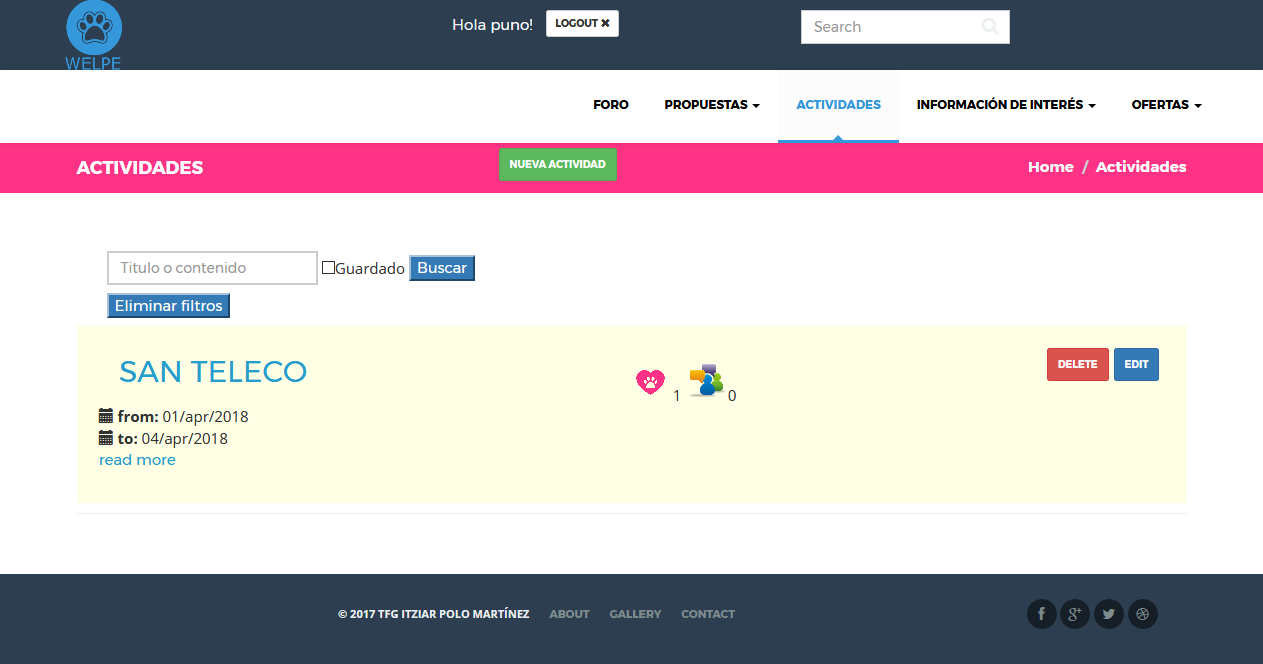
\includegraphics[width=12cm]{img/actividades}
   \caption{Vista de la lista de actividades}
   \label{figura:actividades}
\end{figure}

\subsubsection{Página de una Actividad}
\label{subsubsec:actividad}


La página de una actividad es enviada al cliente cuando se recibe una petición GET sobre el recurso /propuestas/{título\_actividad}


En esta vista se muestra toda la información relativa a la actividad previamente introducida a través del formulario comentado anteriormente. 


Relativo a esta vista, se encuentra el nombre, numero de comentarios, los comentarios, la popularidad de la actividad basada en el número de favoritos, la descripción de la actividad, las fechas, etc.


En esta vista se puede interactuar de las siguientes formas, sólo si es un usuario registrado:



\begin{itemize}
\item Si la actividad incluye que se puedan incluir miniactividades. Se podrá crear miniactividades mediante el botón nueva miniactividad donde se abrirá un modal en el que se pedirán ciertos datos; este formulario ya cumplimentado se enviará al servidor donde se procesará y almacenara. Las miniactividades son actividades dentro de una gran actividad.  
\item Si la actividad proporciona un registro, la vista contendrá una pestaña de registro de usuarios. Donde los usuarios que deseen participar puedan inscribirse. Mientras que los administradores de la actividad pueden además ver y obtener la lista de participantes mediante la descarga de un archivo xls.
\item Se ha proporcionado un apartado de comentarios a la actividad para que los usuarios puedan comentar cada actividad.
\end{itemize}

\begin{figure}[H]
   \centering
   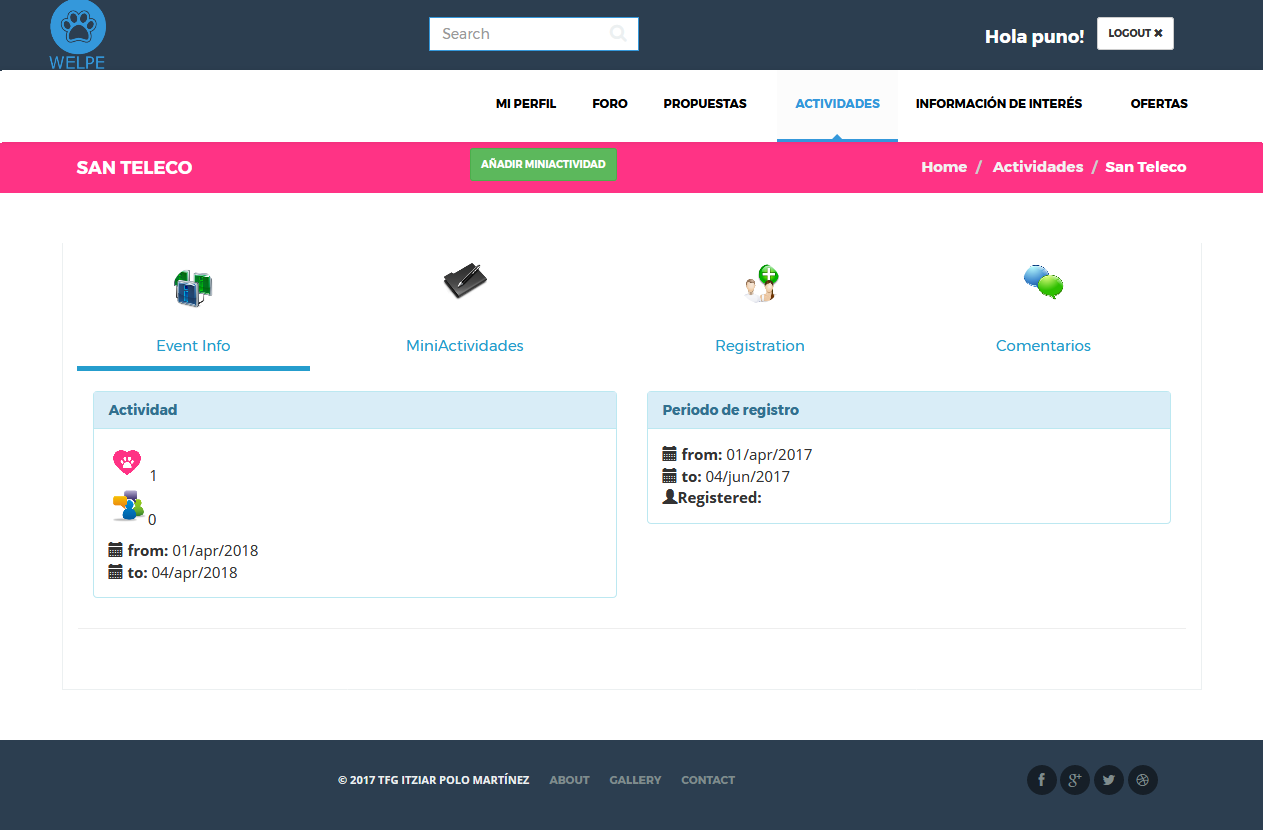
\includegraphics[width=12cm]{img/actividad}
   \caption{Vista de una actividad}
   \label{figura:actividad}
\end{figure}
\begin{figure}[H]
   \centering
   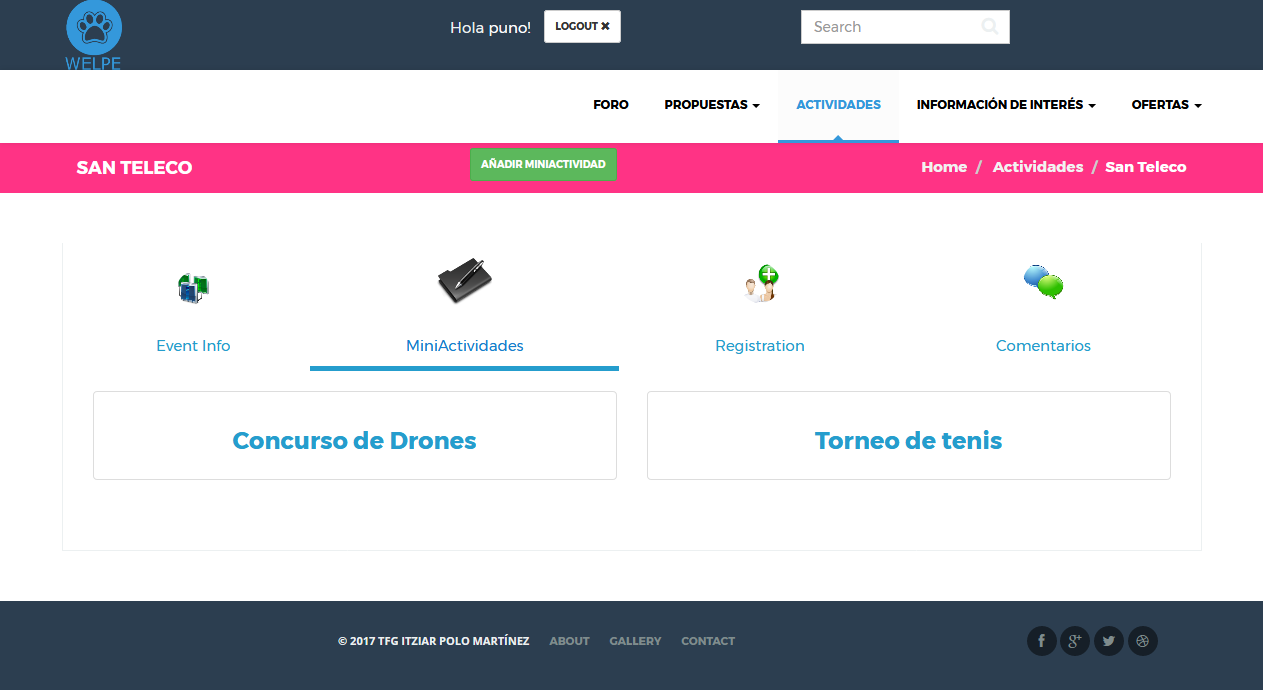
\includegraphics[width=12cm]{img/actividad_miniactividad}
   \caption{Vista de las miniactividades}
   \label{figura:actividad_miniactividad}
\end{figure}
\begin{figure}[H]
   \centering
   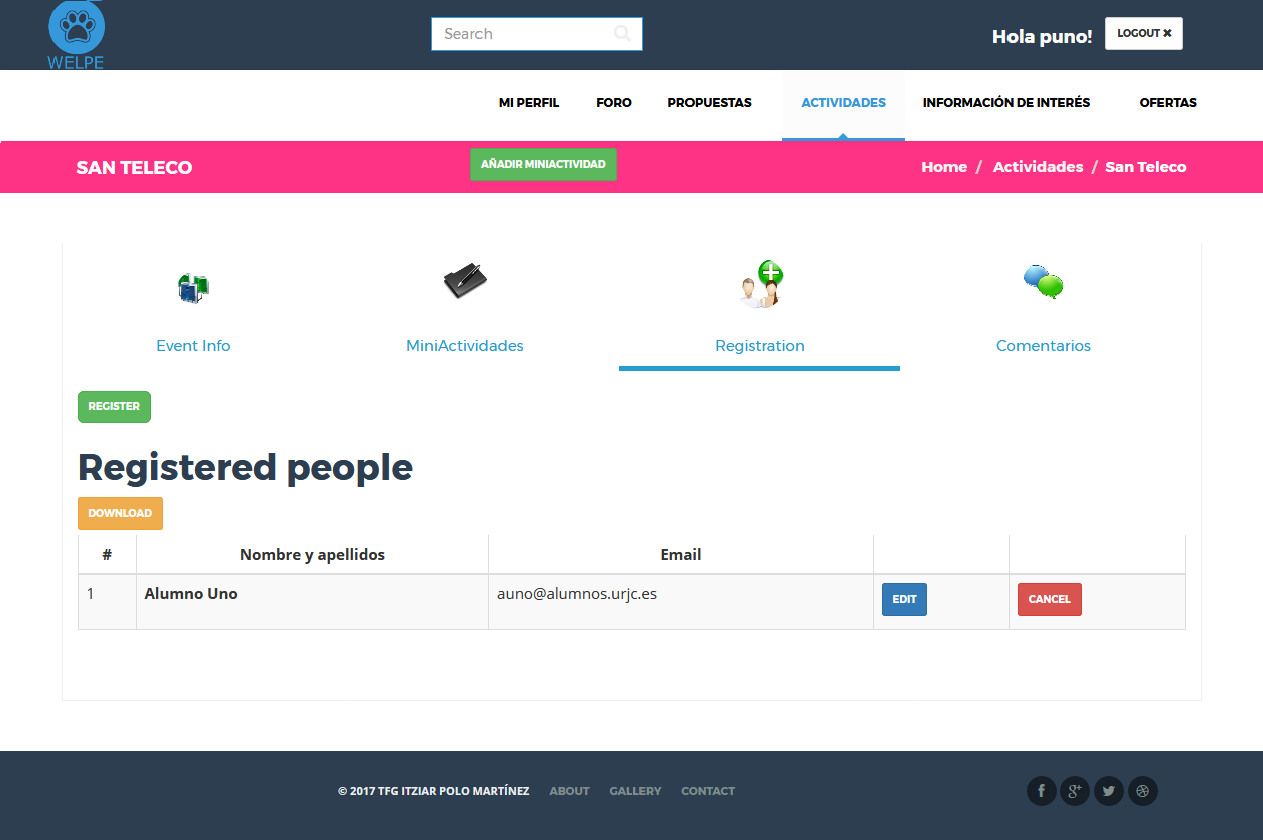
\includegraphics[width=12cm]{img/actividad_registro}
   \caption{Vista del registro}
   \label{figura:actividad_registro}
\end{figure}
\begin{figure}[H]
   \centering
   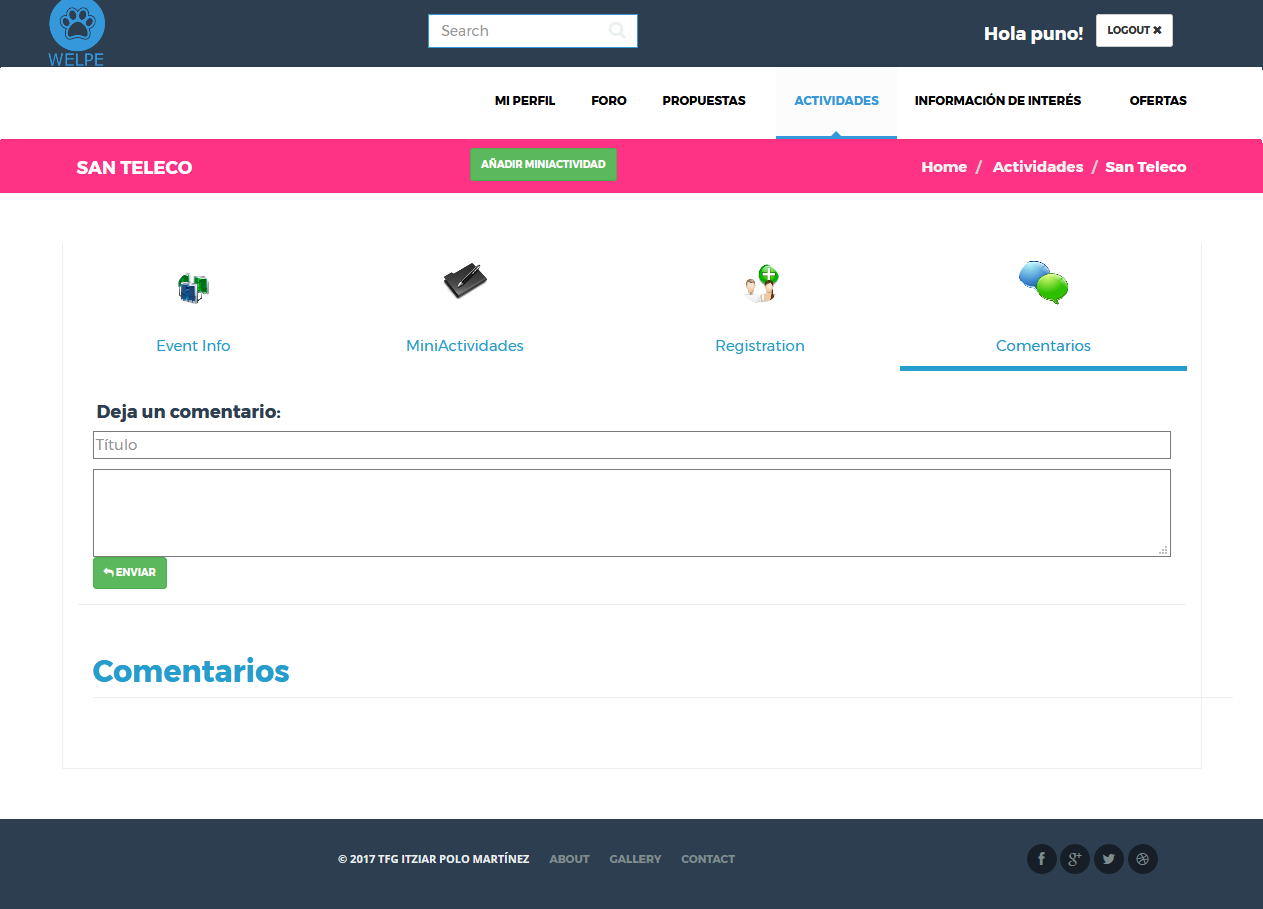
\includegraphics[width=12cm]{img/actividad_comment}
   \caption{Vista de los comentarios a una actividad}
   \label{figura:actividad_comment}
\end{figure}


\subsubsection{Página de Ofertas}
\label{subsubsec:ofertas}


La página del listado de ofertas es enviada al cliente cuando se recibe una petición GET sobre el recurso /ofertas.


En esta vista se muestra un listado con todas las ofertas que se han ido recopilando junto con una pequeña parte de la descripción. Además a la izquierda del título se muestra el tipo de contrato que se ofrece y a la derecha se puede observar varios elementos. En primer lugar un corazón que viene a significar si la oferta se ha guardado en la lista de favoritos o no, además de un número que irá creciendo o decreciendo dependiendo del número de usuarios que guarden en sus listas de favoritos dichas ofertas. A continuación se observa el número de comentarios que contiene cada una de las ofertas.


También cualquier usuario (registrado o no) puede filtrar las ofertas por la/s palabra/s que contenga el título o contenido de la oferta, además también se puede filtrar por el tipo de contrato que se ofrece a elegir entre contrato indefinido, prácticas u otro tipo de contratos y además si el usuario está registrado podrá filtrar si la oferta está o no en su lista de favoritos.


Para introducir una nueva oferta cualquier usuario registrado puede hacerlo. Para ello se rellena el formulario con los datos correspondientes y envía ese formulario. Esta petición llega al servidor mediante una petición POST donde se encargará de sacar los datos y guardarlos correctamente en la base de datos, devolviendo como resultado una nueva vista donde se muestra la nueva oferta.


Por último, sólo si el usuario ha creado una determinada oferta o es un profesor o es el administrador: podrá modificar y/o eliminar dicha oferta mediante los botones edit y delete.


\begin{figure}[H]
   \centering
   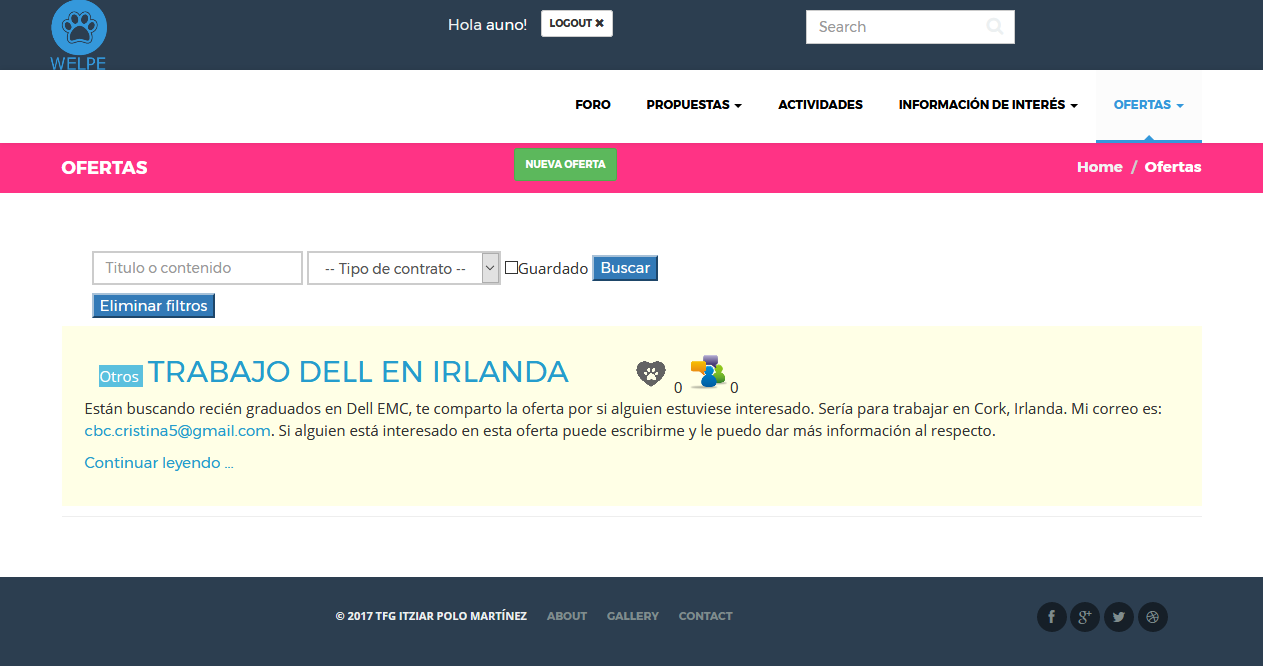
\includegraphics[width=12cm]{img/ofertas}
   \caption{Vista de la lista de ofertas}
   \label{figura:ofertas}
\end{figure}


\subsubsection{Página de una Oferta}
\label{subsubsec:oferta}


La página de una oferta es enviada al cliente cuando se recibe una petición GET sobre el recurso /ofertas/{título\_oferta}


En esta vista se muestra toda la información relativa a la oferta previamente introducida a través del formulario comentado anteriormente. 


Relativo a esta vista se encuentra el nombre, el tipo de contrato ofertado, número de comentarios, los comentarios, las veces que la oferta se ha guardado en la lista de favoritos, la descripción de la oferta, como aplicar a la oferta, etc.


En esta vista se puede interactuar de las siguientes formas sólo si el usuario registrado:


\begin{itemize}
\item Se puede crear una nueva oferta mediante el botón nueva oferta donde se abrirá un modal en el que se pedirán ciertos datos; este formulario ya cumplimentado se enviará al servidor donde se procesará y almacenara, devolviendo como resultado una nueva vista donde se muestra la oferta que el usuario previamente ha creado.
\item Si el usuario es el propietario de la oferta podrá modificarla mediante el botón edit y también podrá eliminarla mediante el botón eliminar.
\item •	Junto con todo ello, está también el botón de favoritos donde el usuario puede agregar o eliminar la oferta de su lista de favoritos.  
\item Se ha proporcionado un apartado de comentarios a la oferta para que los usuarios puedan comentar cada oferta.
\end{itemize}


\begin{figure}[H]
   \centering
   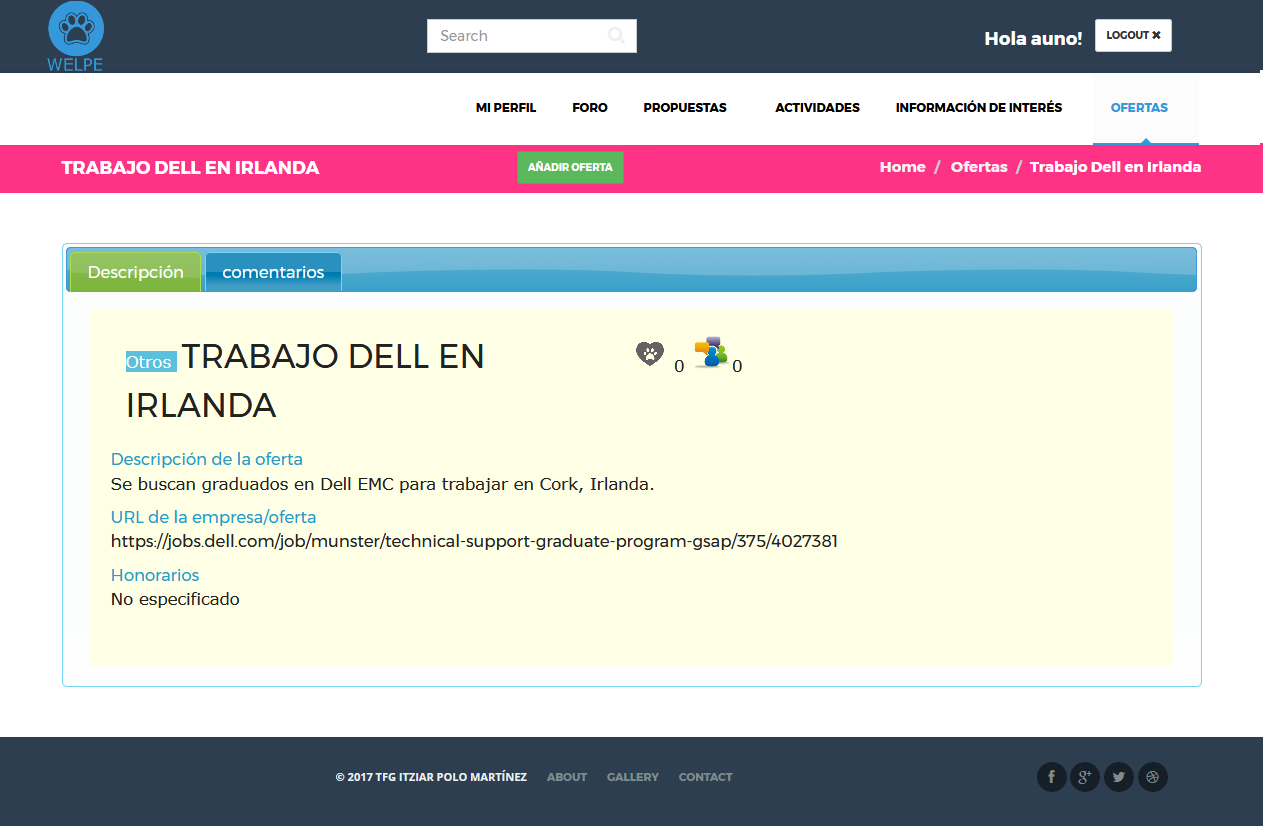
\includegraphics[width=12cm]{img/oferta}
   \caption{Vista de una oferta}
   \label{figura:oferta}
\end{figure}
\begin{figure}[H]
   \centering
   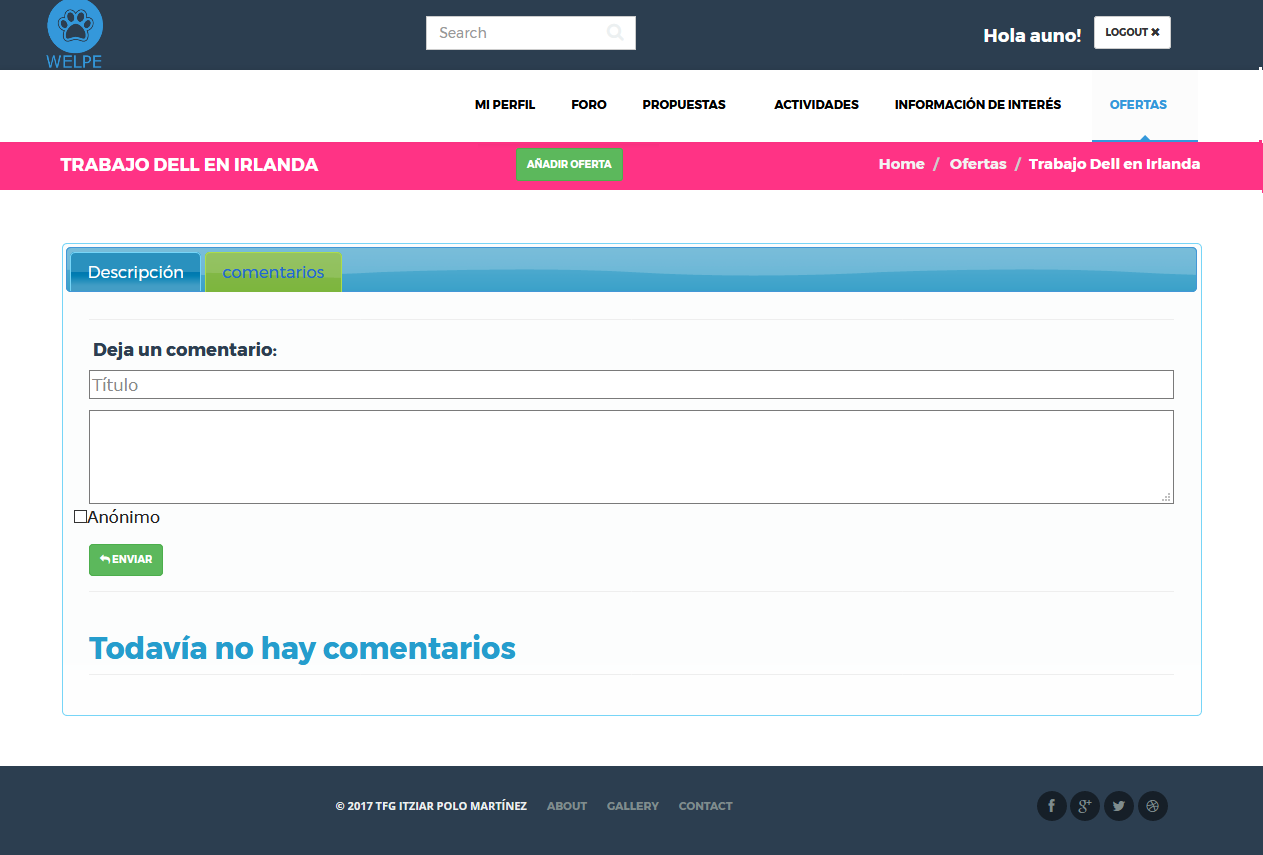
\includegraphics[width=12cm]{img/oferta_comment}
   \caption{Vista de los comentarios a una oferta}
   \label{figura:oferta_comment}
\end{figure}


\subsubsection{Página de Información de Interés}
\label{subsubsec:informaciones}


La página del listado de informaciones es enviada al cliente cuando se recibe una petición GET sobre el recurso /informacion.


En esta vista se muestra un listado con toda la información de las distintas informaciones de interés que se han ido recopilando junto con una pequeña parte de la descripción. Además a la izquierda del título se muestra la clase de información que ofrece y a la derecha se puede observar varios elementos. En primer lugar un corazón que viene a significar si la información de interés se ha guardado en la lista de favoritos o no, además de un número que irá creciendo o decreciendo dependiendo del número de usuarios que las guarden en sus listas de favoritos. A continuación se observa el número de comentarios que contiene cada información.


También cualquier usuario (registrado o no) puede filtrar este listado por la/s palabra/s que contenga el título o contenido de la información deseada, además también podemos filtrar por el tipo de información que se ofrece a elegir entre beca de estudios, programa, curso, concurso u otro tipo de información y además si el usuario está registrado podrá filtrar si la información está o no en su lista de favoritos.


Para introducir una nueva información cualquier usuario registrado puede hacerlo. Para ello se hace click en el botón “Añadir información” se rellena el formulario con los datos correspondientes y se envía. Esta petición llega al servidor mediante una petición POST donde se encargará de sacar los datos y guardarlos correctamente en la base de datos devolviendo como resultado una nueva vista donde se muestra la información de interés que el usuario previamente había enviado.


Por último, sólo si el usuario ha creado una determinada información de interés o es un profesor o es el administrador: podrá modificar y/o eliminar dicha información mediante los botones edit y delete.

\begin{figure}[H]
   \centering
   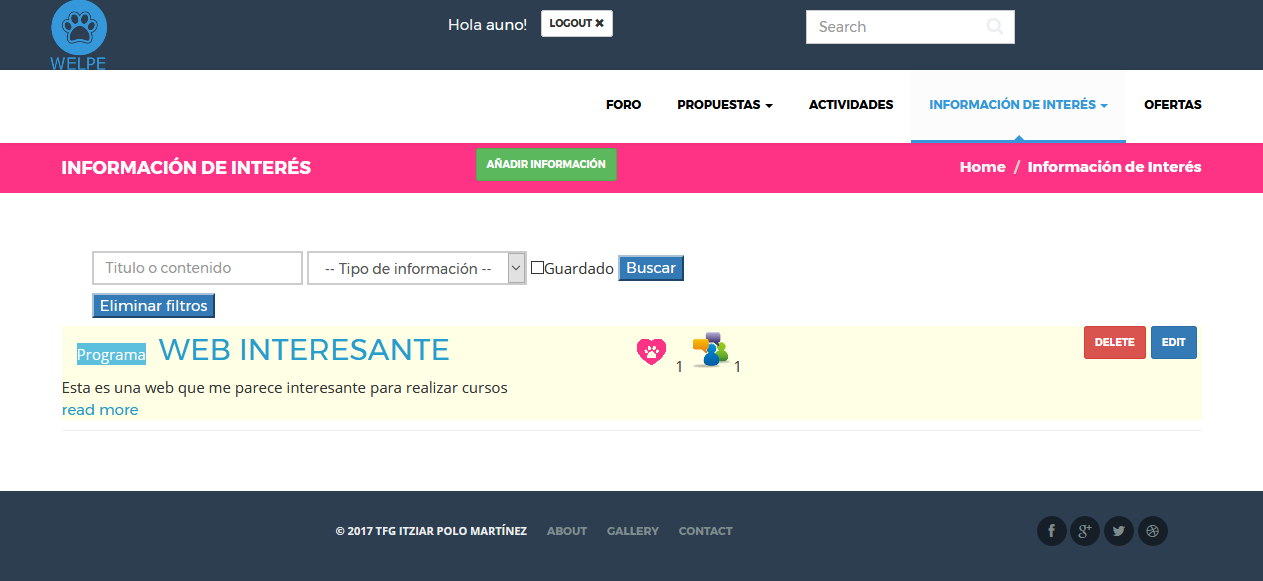
\includegraphics[width=12cm]{img/infos_interes}
   \caption{Vista de la lista de informaciones de interés}
   \label{figura:infos_interes}
\end{figure}



\subsubsection{Página de una Información de interés }
\label{subsubsec:informacion}


La página de una información es enviada al cliente cuando se recibe una petición GET sobre el recurso /informacion/{título\_información\_de\_interés}


En esta vista se muestra toda la información relativa a una única información de interés que previamente ha sido incluida a través del formulario comentado anteriormente. 


Relativo a esta vista se encuentra el título, el tipo de información ofrecida, número de comentarios, los comentarios, las veces que dicha información de interés se ha guardado en la lista de favoritos, la descripción de la información, url donde encontrar más información, etc.


En esta vista se puede interactuar de las siguientes formas sólo si es un usuario registrado:



\begin{itemize}
\item Se puede crear una nueva información  mediante el botón añadir información donde se abrirá un modal en el que se pedirán ciertos datos, este formulario ya cumplimentado se enviará al servidor donde se procesará y almacenará devolviendo como resultado una nueva vista donde se muestra la nueva información de interés.
\item Si el usuario es el propietario de la información de interés podrá modificar mediante el botón edit, y eliminarla mediante el botón delete.
\item Junto con todo ello, está también el botón de favoritos donde el usuario puede agregar o eliminar dicha información de interés de su lista de favoritos.  
\item Se ha proporcionado un apartado de comentarios donde los usuarios pueden compartir sus opiniones y/o aclarar sus dudas acerca de la información de interés.
\end{itemize}


\begin{figure}[H]
   \centering
   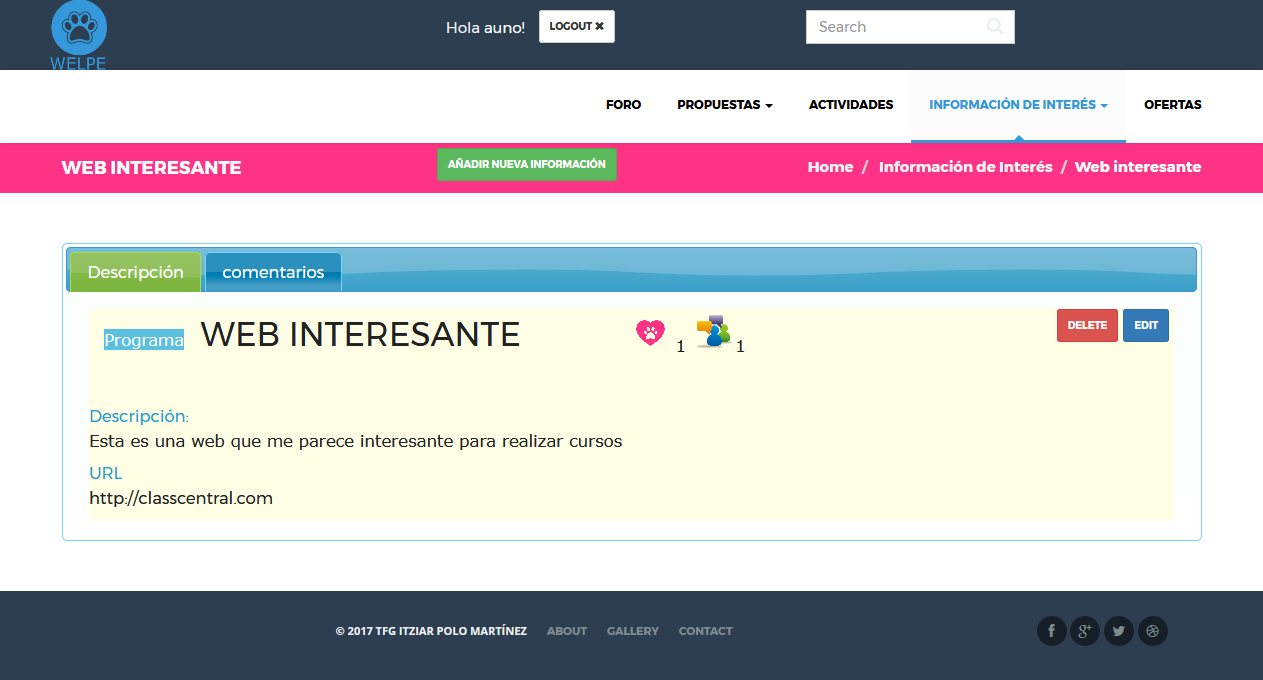
\includegraphics[width=12cm]{img/info_interes}
   \caption{Vista de una información de interés}
   \label{figura:info_interes}
\end{figure}
\begin{figure}[H]
   \centering
   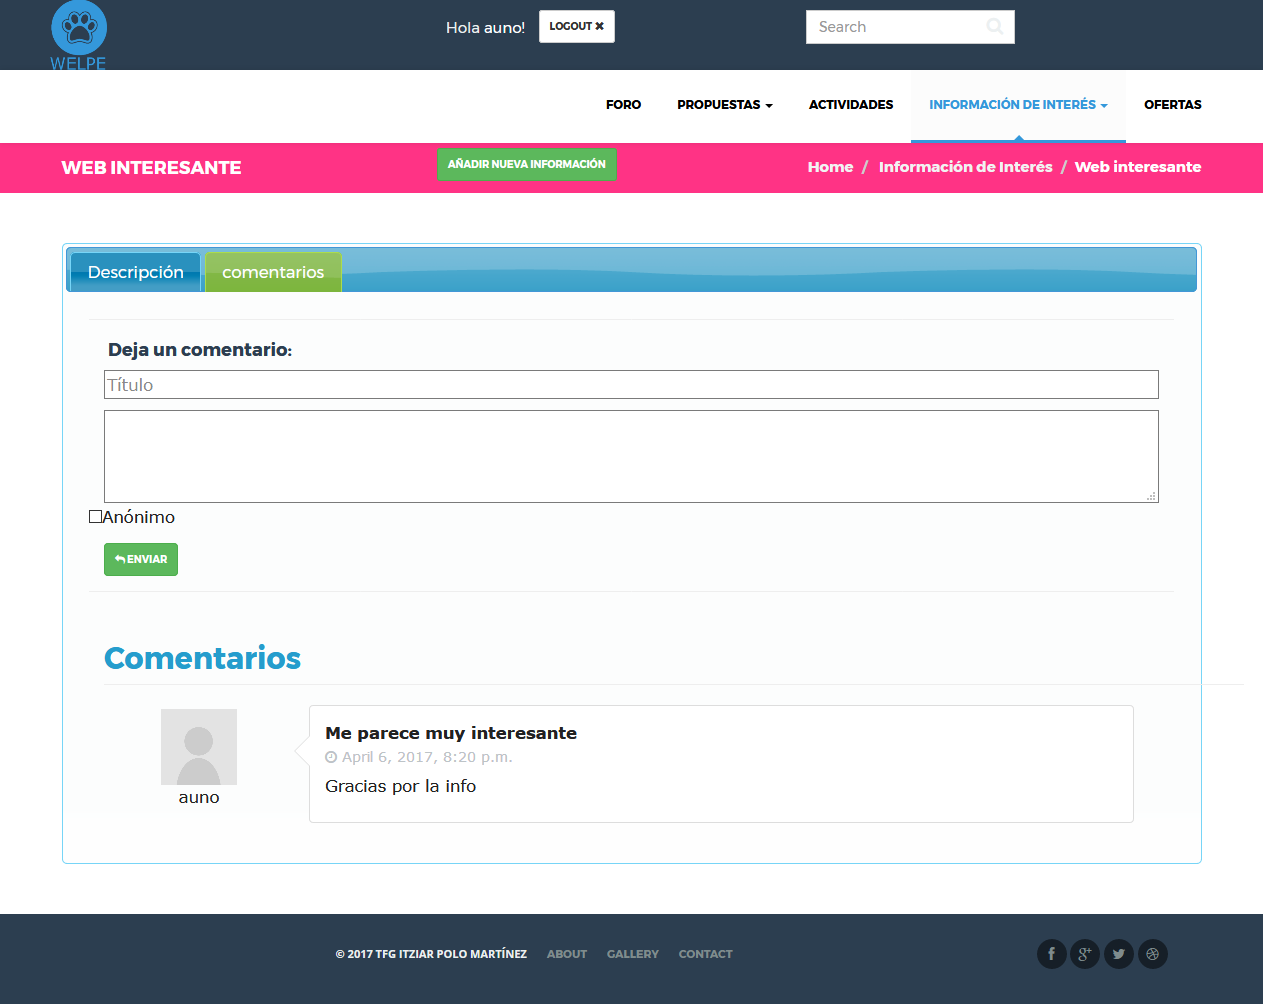
\includegraphics[width=12cm]{img/info_interes_comment}
   \caption{Vista de los comentarios a una información de interés}
   \label{figura:info_interes_comment}
\end{figure}

\subsubsection{Página de Política de Cookies}
\label{subsubsec:cookies}


Esta vista tiene que ver más con la legislación que con la propia aplicación.


El Real Decreto-ley 13/2012, de 30 de marzo, publicado en el «Boletín Oficial del Estado» el pasado sábado 31 de marzo de 2012, transpone la Directiva 2009/136/CE, del Parlamento Europeo y del Consejo, de 25 de noviembre de 2009, que se integra en la LSSI (Ley 34/2002, de 11 de julio, de servicios de la sociedad de la información y de comercio electrónico) modificando el punto segundo de su artículo 22, que queda redactado de la forma siguiente:


``Artículo 22.2 de la Ley 34/2002. Los prestadores de servicios podrán utilizar dispositivos de almacenamiento y recuperación de datos en equipos terminales de los destinatarios, a condición de que los mismos hayan dado su consentimiento después de que se les haya facilitado información clara y completa sobre su utilización, en particular, sobre los fines del tratamiento de los datos, con arreglo a lo dispuesto en la Ley Orgánica 15/1999, de 13 de diciembre, de Protección de Datos de Carácter Personal. Cuando sea técnicamente posible y eficaz, el consentimiento del destinatario para aceptar el tratamiento de los datos podrá facilitarse mediante el uso de los parámetros adecuados del navegador o de otras aplicaciones, siempre que aquél deba proceder a su configuración durante su instalación o actualización mediante una acción expresa a tal efecto. Lo anterior no impedirá el posible almacenamiento o acceso de índole técnica al solo fin de efectuar la transmisión de una comunicación por una red de comunicaciones electrónicas o, en la medida que resulte estrictamente necesario, para la prestación de un servicio de la sociedad de la información expresamente solicitado por el destinatario.''


Por si no hubiera quedado claro del todo nos podríamos enfrentar a distintas sanciones dependiendo de la gravedad que consideren:


\begin{itemize}
\item Sanción Leve hasta 30.000 Euros.  Art. 38.4 LSSI. Son infracciones leves:
g) ``El incumplimiento de las obligaciones de información o de establecimiento de un procedimiento de rechazo del tratamiento de datos, establecidas en el apartado 2 del artículo 22, cuando no constituya una infracción grave.''
\item Sanción Grave de 30.000 hasta 150.000 Euros. Art. 38.3 LSSI. Son infracciones graves:
i) ``El incumplimiento significativo de las obligaciones de información o de establecimiento de un procedimiento de rechazo del tratamiento de datos, establecidas en el apartado 2 del artículo 22.''
\end{itemize}


Con lo cual lo más conveniente es informar al usuario para evitar posibles sanciones.
 

\subsubsection{Páginas de Sitemaps}
\label{subsubsec:sitemap}


Para mejorar el posicionamiento SEO, una recomendación es  tener dos sitemaps, uno para los buscadores (se puede acceder a través de /sitemap.xml) y otro creado especialmente para la compresión humana (se puede acceder a través de /sitemap).


El primero de los sitemap (sitemap.xml) el cms que se utiliza (Mezzanine) lo crea por defecto.


El segundo (/sitemap), se ha creado especialmente una aplicación mostrar el recorrido del árbol.


\subsubsection{Vista del panel de administración}
\label{subsubsec:admin}


Mezzanine al igual que Django, ofrece unas vistas para administrar la base de datos que es muy útil y fácil de usar. Desde ahí se puede crear, modificar o eliminar cualquier elemento que se desee y hacer un seguimiento de la base de datos. 


Cada aplicación creada en este proyecto junto con otras, que el propio CMS posee, se encuentran disponibles en la parte de administración.  


Podemos observar que además de las vistas explicadas anteriormente también podemos podemos crear otras que ya vienen predefinadas con Mezzanine como entradas para un Blog, un Page (que sería como una página simple).


Además tenemos otras configuraciones sobre la plataforma en sí, como las proporcionadas por los menus Site y Theme.


Esta vista sólo es accesible para los administradores de la plataforma. Se puede acceder a ella a través de /admin.
